\documentclass{beamer}
\usepackage[spanish, english]{babel}
\selectlanguage{spanish}
\usepackage[fixlanguage]{babelbib}
\selectbiblanguage{spanish}
\usepackage{graphicx}
\usepackage[utf8]{inputenc}%Para poder usar acentos y otras letras latinas del español
\usepackage[T1]{fontenc}
\usepackage{verbatim}%comments

\usepackage{caption, subcaption}

\bibliographystyle{bababbrv}

\usetheme{Darmstadt}

\title{Clasificación de Razas}
\subtitle{De Perros y Gatos}


\author[Bahamonde, Gonz\'alez]{J.~Bahamonde\inst{1} \and S.~Gonz\'alez\inst{1}}
\institute[University de Chile]
{
	\inst{1}
	Departamento de las Ciencias de la Computaci\'on\\
	Universidad de Chile
}

\begin{document}
\begin{frame}[label=firstframe]
      \titlepage % (Or whatever else goes here.)
\end{frame}
\begin{frame}{El problema}
    El determinar automáticamente razas y especies de animales y plantas
    aparece en diversos contextos:
    \pause
    \begin{itemize}
        \item Monitorear automáticamente las poblaciones de aves en un parque forestal.
            \pause 
        \item Determinar la especie de una flor a partir de su fotografía
            puede servir a herboristas en el campo.
            \pause
        \item La detección automática de razas de animales puede servir de
            apoyo a veterinarios, o a buscar animales perdidos.
    \end{itemize}
    \pause
    \begin{center}
        
\includegraphics[scale=0.4]{imagen/asirra}
        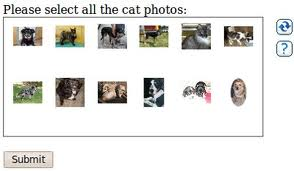
\includegraphics[scale=0.4]{imagen/asirraT}
    \end{center}
\end{frame}
\begin{frame}{El problema}
    %CONTENT
    \begin{itemize}
        \item El problema de clasificación entre clases muy disimilares ha
            sido ampliamente estudiado.
            \pause
        \item El dataset Caltech presenta el problema de discriminar el
            Golden Gate con una iguana.
            \begin{center}
                {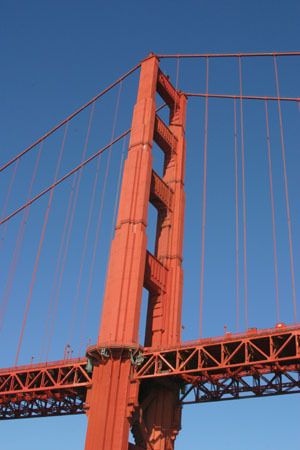
\includegraphics[scale=0.2]{imagen/ggate.jpg}}
                {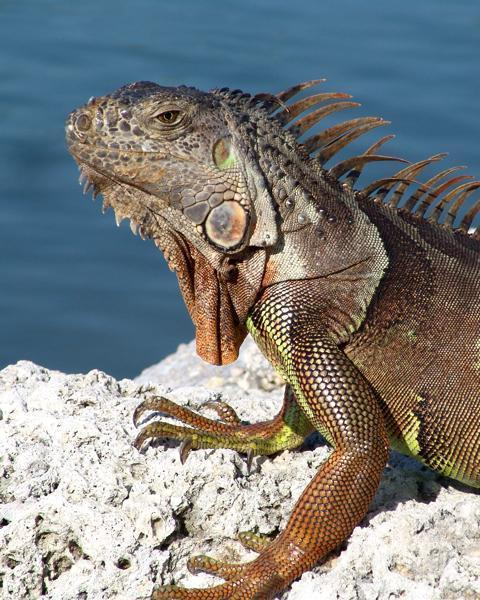
\includegraphics[scale=0.14]{imagen/iguana.jpg}}
            \end{center}
            \pause
        \item Por otro lado, discriminar entre clases muy similares (razas,
            especies) es \textbf{categorización fina de objetos}
            \textit{(fine grained object categorization)}. 
    \end{itemize}
\end{frame}
\begin{frame}{El problema}
    %CONTENT
    \begin{itemize}
        \item En particular, perros y gatos poseen un buen
            grado de variabilidad.
    \end{itemize}
    \pause
    \begin{center}
        {
\includegraphics[scale=0.2]{imagen/fitsisits.jpg}}
        {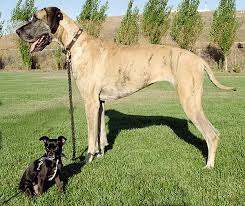
\includegraphics[scale=0.5]{imagen/dogdiff.jpg}}
    \end{center}
\end{frame}	

\begin{frame}{Funcionamiento de la solución}
    Dada una imagen donde aparece un animal (gato o perro), identificar la
    especie y raza a la que pertenece.
\end{frame}

\begin{frame}{Propuesta de solución}
    \begin{itemize}
        \item Separar el animal del fondo (\emph{segmentación})
            \pause
            \begin{center}
                \raisebox{-.5\height}{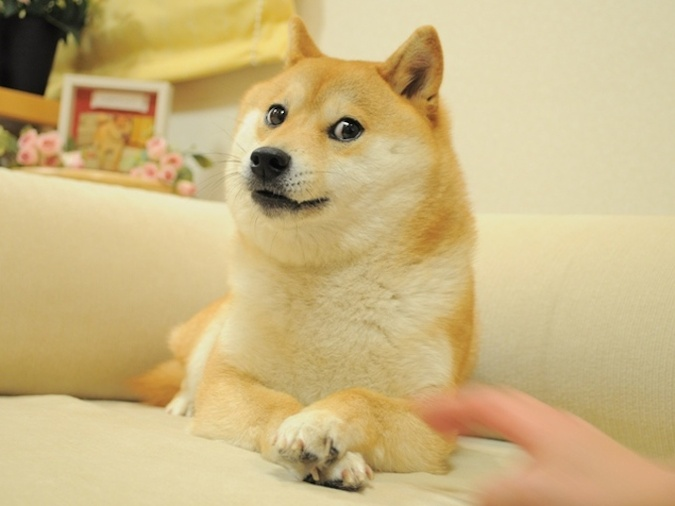
\includegraphics[scale=0.1]{imagen/doge}}
                \pause
                $\implies$
                \raisebox{-.5\height}{
\includegraphics[scale=0.1]{imagen/doge_segmentation}}
            \end{center}
            \pause
            \ \\ 
        \item Discriminar especie y raza sobre el animal aislado
            \pause
            \begin{center}
                \raisebox{-.5\height}{
\includegraphics[scale=0.1]{imagen/doge_segmentation}}
                \pause
                $\implies$
                {``Shiba Inu''\ \ \ \ \ \ }
            \end{center}
    \end{itemize}
\end{frame}

\begin{frame}{Estado del Arte: Gatos y Perros \footnote{\emph{Cats and
    Dogs}, Parkhi, Vedaldi, Zisserman y Jawahar, 2012.}}
    \begin{itemize}
            \pause
        \item Modelo de partes deformables (HOG + resortes).
            \pause
        \item Segmentación automática mediante \emph{grab-cut}.
            \pause
        \item \emph{Bag-of-words} con descriptores SIFT. 
            \pause
    \end{itemize}
    \begin{center}
        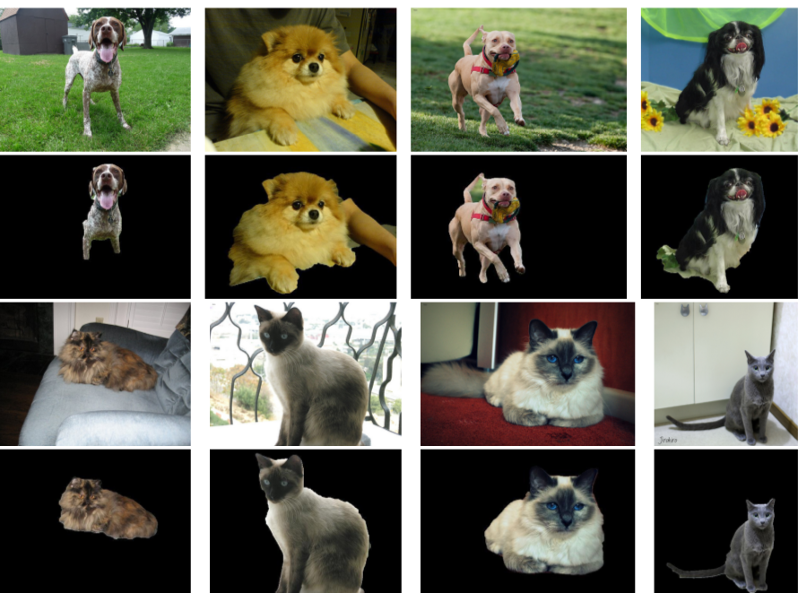
\includegraphics[scale=0.2]{imagen/parkhi}
    \end{center}
\end{frame}

\begin{frame}{Estado del Arte: Clasificación de Razas de
        Perros\footnote{\emph{Dog Breed Classification Using Part
    Localization}, Liu, Kanazawa, Jacobs y Belhumeur, 2012. }}
    \begin{itemize}
            \pause
        \item Detección de cara del perro.
            \pause
        \item Identificación de partes.
            \pause
        \item Histograma de color y descriptores SIFT en torno a las partes.
            \pause
    \end{itemize}
    \begin{center}
        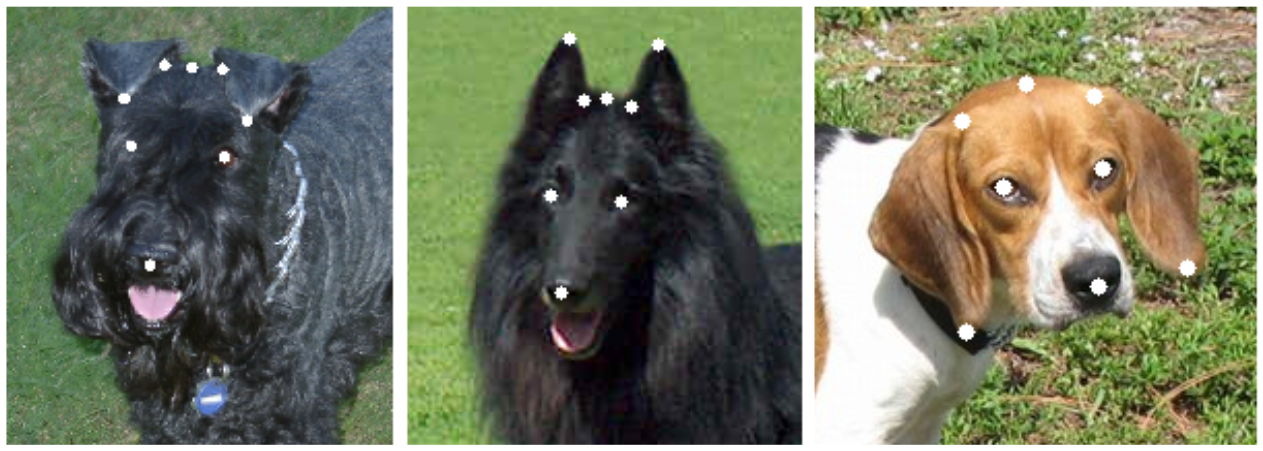
\includegraphics[scale=0.15]{imagen/dogannotation}
    \end{center}
\end{frame}
\begin{frame}{Estado del Arte: Detección de Gatos \footnote{\emph{Cat Head
            Detection - How to Effectively Exploit Shape and Texture Features},
    Zhang, Sun, Tang, 2008}}
    \begin{itemize}
            \pause
        \item No es clasificación, sino que detección.
            \pause
        \item Entrenan dos detectores con \emph{datasets} normalizados de
            distinta forma.
            \pause
        \item Un clasificador fusiona la información de ambos para decidir
            si está frente a un gato o no.
            \pause
    \end{itemize}
    \begin{center}
        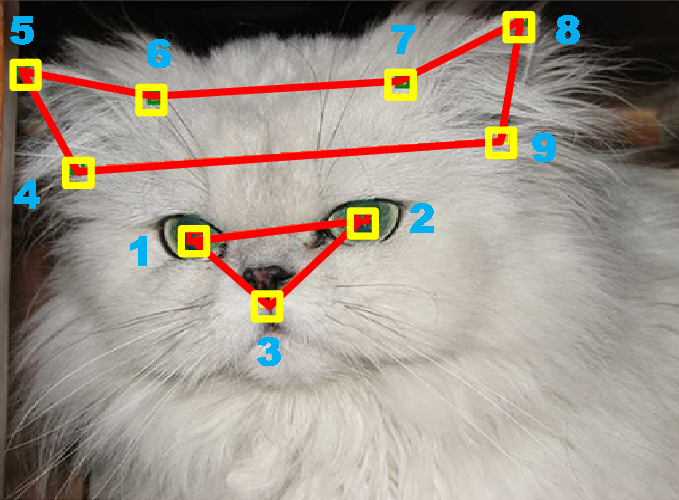
\includegraphics[scale=0.25]{imagen/annotation}
    \end{center}
\end{frame}

\begin{frame}{Nuestra aproximación}
    \begin{itemize}
        \item Utilizar \emph{grab-cut} para la segmentación.
            \pause
        \item Utilizar descriptores de textura para la posterior
            clasificación.
    \end{itemize}
\end{frame}
\begin{frame}{Evaluación}
    \begin{itemize}
        \item Primera etapa: gatos vs. perros $\implies$ ROC.
            \pause
        \item Segunda etapa: razas $\implies$ matriz de confusión.
    \end{itemize}
\end{frame}
\begin{frame}{Dataset}
    \begin{itemize}
        \item $\approx 7400$ imágenes de 25 razas de perros y 12 de gatos
            ($\approx 200$ por raza).
            \pause
        \item Anotaciones de forma y raza.
            \pause
            \begin{center}
                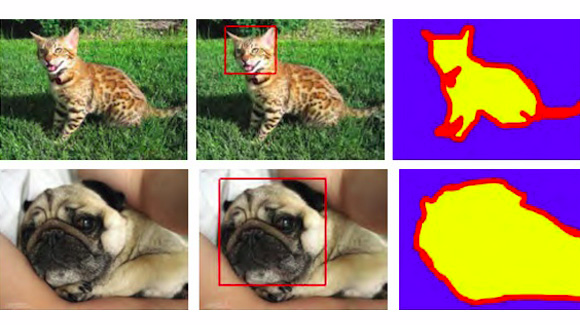
\includegraphics[scale=0.3]{imagen/catsanddogs_annotation}
            \end{center}
    \end{itemize}
\end{frame}

\againframe{firstframe}
%COMENTARIO INICIA ACA=================================================================================================
\begin{comment}

    \begin{frame}
        \frametitle{Estado del Arte.}
        %CONTENT
        \selectlanguage{spanish}
        \selectbiblanguage{spanish}
        \bibliography{./presentation}
    \end{frame}
    \begin{frame}
        \frametitle{Reconocimiento facial de gatos.}
        %CONTENT
        \url{http://harthur.github.io/kittydar/}

        Utiliza método propuesto en \emph{Cat head detection-how to effectively exploit shape and texture features}\cite{zhang2008cat}
        \begin{figure}[H]
            \centering
            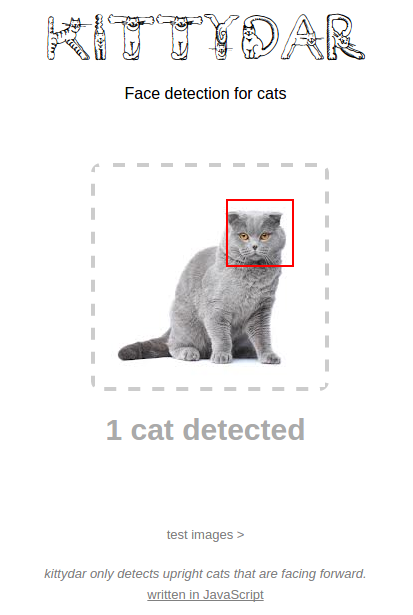
\includegraphics[scale=0.27]{imagen/Captura.png}
        \end{figure}
    \end{frame}
    \begin{frame}
        \frametitle{Reconocimiento facial de gatos.}
        %CONTENT
        Comparación entre métodos.
        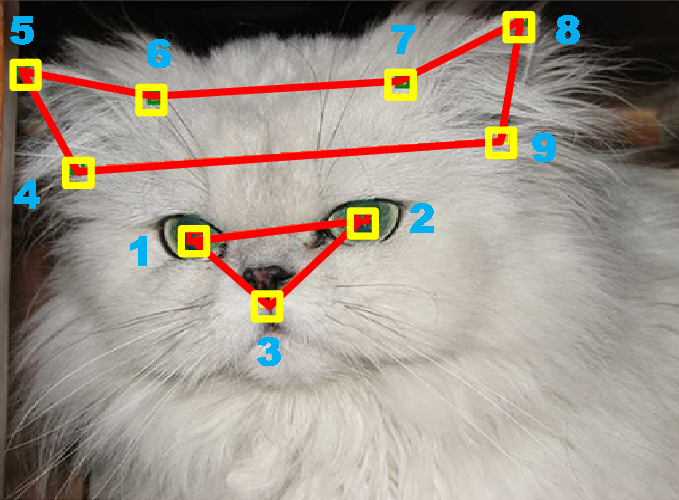
\includegraphics[scale=0.15]{imagen/annotation.png}
        \begin{itemize}
            \item{
                    HOG.
                }
            \item{
                    Haar.
                }
            \item{
                    Detección de formas y textura conjunta.
                }
        \end{itemize}
        \begin{figure}[H]
            \centering
            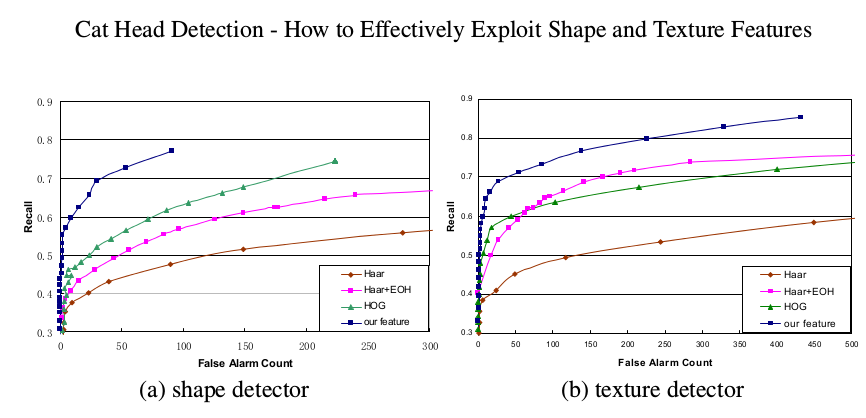
\includegraphics[scale=0.30]{imagen/cat-roc.png}
        \end{figure}
    \end{frame}
    \begin{frame}
        \frametitle{Resultados}
        %CONTENT
        \begin{figure}[H]
            \centering
            \subcaptionbox{}{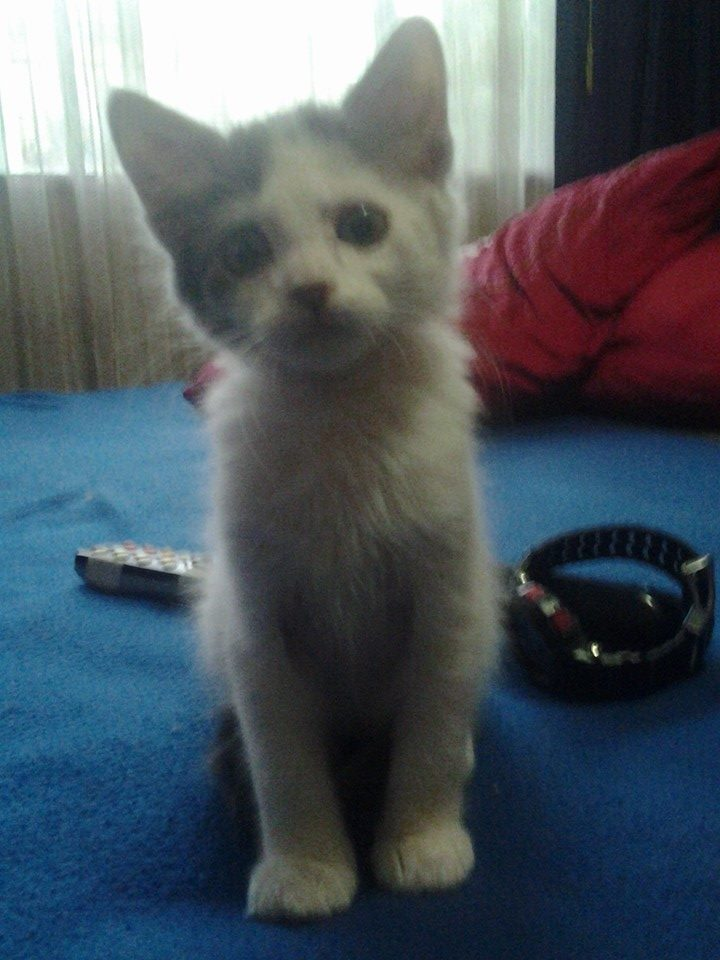
\includegraphics[scale=0.07]{imagen/nw1.jpg}}
            \subcaptionbox{}{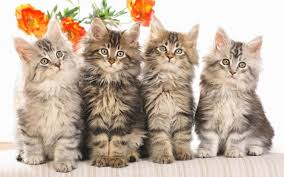
\includegraphics[scale=0.38]{imagen/nw2.jpg}}
            \subcaptionbox{}{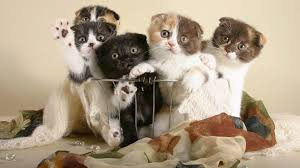
\includegraphics[scale=0.39]{imagen/nw3.jpg}}
            \caption{No reconoce gatitos.}
        \end{figure}
    \end{frame}
    \begin{frame}
        \frametitle{Resultados}
        %CONTENT
        \begin{figure}[H]
            \centering
            \subcaptionbox{}{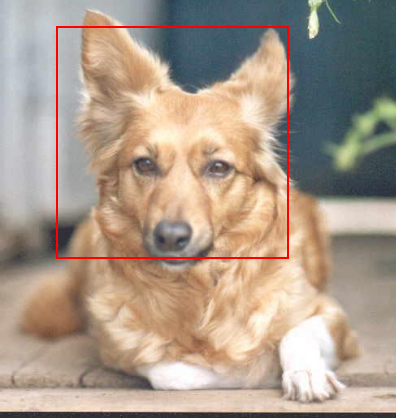
\includegraphics[scale=0.3]{imagen/w1.png}}
            \subcaptionbox{}{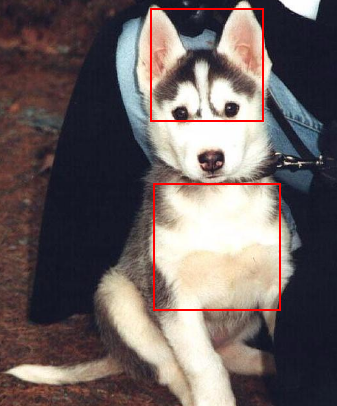
\includegraphics[scale=0.31]{imagen/w2.png}}
            \caption{Reconoce algunos perros.}
        \end{figure}
    \end{frame}
    \begin{frame}
        \frametitle{Resultados}
        %CONTENT
        \begin{figure}[H]
            \centering
            \subcaptionbox{}{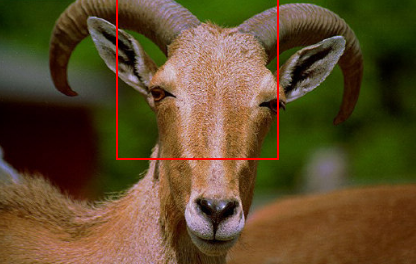
\includegraphics[scale=0.27]{imagen/f1.png}}
            \subcaptionbox{}{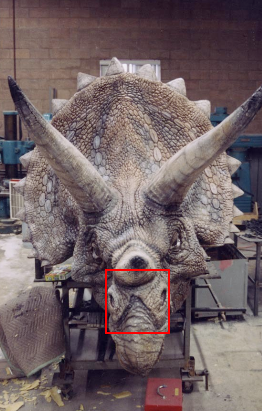
\includegraphics[scale=0.28]{imagen/f2.png}}
            \subcaptionbox{}{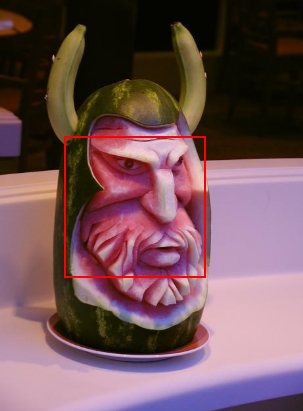
\includegraphics[scale=0.28]{imagen/f3.png}}
            \caption{Reconoce... cosas.}
        \end{figure}
    \end{frame}
    \begin{frame}
        \frametitle{Clasificación en Razas de Gatos y Perros.}
        %CONTENT
        \emph{Cats and Dogs}.\cite{parkhi12a}
        \begin{itemize}
            \item{
                    HOG para reconocimiento de \emph{Forma}.
                }
            \item{
                    \emph{Bag of Words} para reconocimiento de \emph{textura}.
                }
        \end{itemize}
        Combinaciones de Rostro, Cuerpo y Fondo.
        \begin{figure}[H]
            \centering
            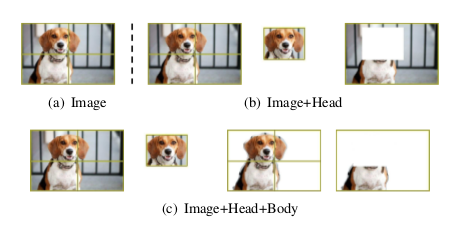
\includegraphics[scale=0.50]{imagen/faceheadimage.png}
        \end{figure}
    \end{frame}
    \begin{frame}
        \frametitle{Clasificación en Razas de Gatos y Perros.}
        %CONTENT
        \begin{figure}[H]
            \centering
            {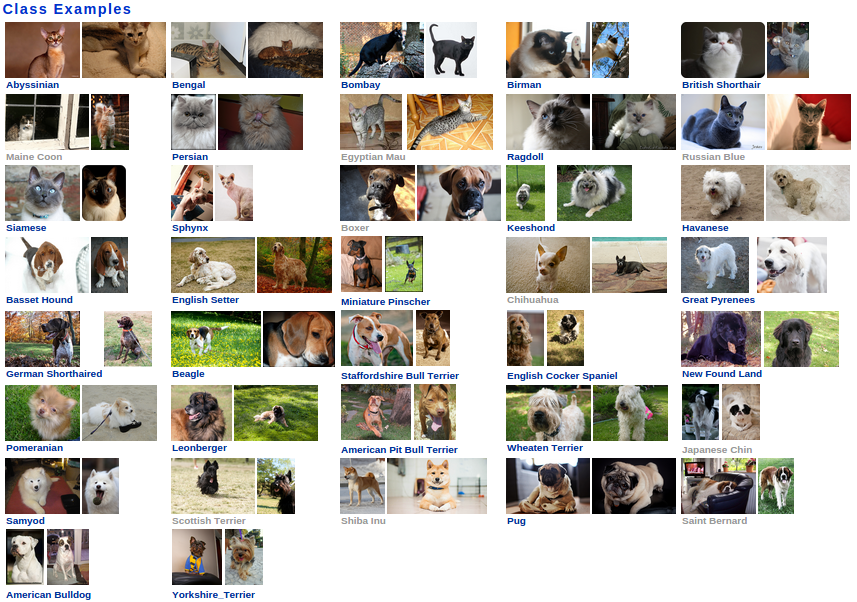
\includegraphics[scale=0.27]{imagen/datasetEx.png}}
            \caption{Dataset de razas de Perros y Gatos.}
        \end{figure}
    \end{frame}
    \begin{frame}
        \frametitle{Reconocimiento facial de Perros.}
        %CONTENT
        \emph{Biometric Recognition for Pet Animal}.\cite{kumar2014biometric}

        PCA \& Eigenfaces.
    \end{frame}
    \begin{frame}
        \frametitle{Reconocimiento facial de Perros.}
        %CONTENT
        \begin{figure}[H]
            \centering
            {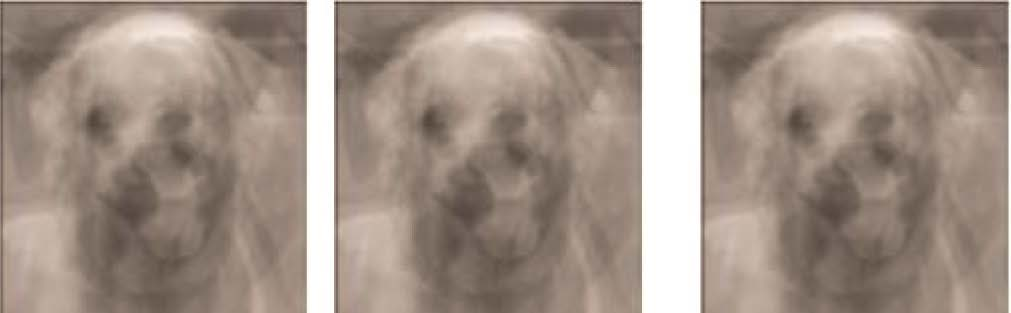
\includegraphics[scale=0.27]{imagen/dogaverage.png}}
            \caption{Eigenfaces para Perros.}
        \end{figure}
    \end{frame}

    %COMENTARIO TERMINA ACA ==============================================================================
\end{comment}
\end{document}
